\documentclass[12pt]{exam}
\usepackage{xparse}
\usepackage{rosoff-vector-macros}
\usepackage{rosoff}
\usepackage{graphicx}
\DeclareGraphicsExtensions{.jpg, .png}
\usepackage{fourier}
\usepackage{MnSymbol}
\usepackage{amsthm}
\usepackage{paralist,enumerate,listings}
\usepackage{siunitx}
\frenchspacing
\usepackage{parskip}
\usepackage{hyperref}
\firstpageheader{}{}{}
\runningheader{\textbf{Fall 2013}}
 {}
 {\textbf{Math 251}}
 %{\emph{Page \thepage~of \numpages}}
\runningheadrule

\pagestyle{head}

\begin{document}
\noindent
\textbf{{\large Math 251 \hfill Quiz 07 (WeBWorK 10)}}
% \hfill Name: \underline{\hspace{0.5in}Answers\hspace{2in}}

\noindent
November 20, 2013; 10 minutes \hfill Name: \underline{\hspace{3in}} 

\noindent

\noindent
This quiz is \emph{open-note}, but no books or calculators may be used.
In calculation, you can show work at your discretion, but remember that
I can't give partial credit for calculations I can't see. Explain
anything that seems to need explaining.

\begin{questions} 

\question[8] Suppose $R$ is the shaded region in the figure. 

\begin{figure}[!h]
    \begin{minipage}[t]{0.3\textwidth}
        \vspace{0pt}
        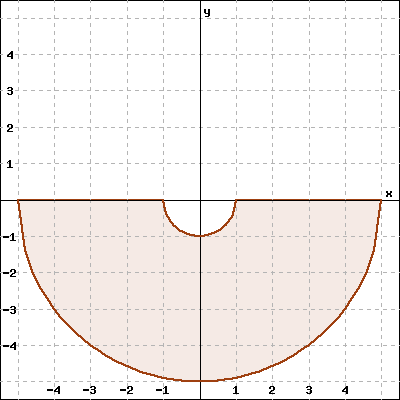
\includegraphics[width=\linewidth]{images/region.png}
    \end{minipage} \hfill
    \begin{minipage}[t]{0.6\textwidth}
        \vspace{0pt}
        As an iterated integral in polar coordinates,
        \begin{equation*}
            \int \!\!\!\!\!\! \int_R f(x,y)\; dA = \int_A^B \int_C^D f(r,\theta) r \; dr \; d\theta
        \end{equation*}
        with limits of integration
        \begin{parts}
            \part $A= $
            \part $B= $
            \part $C= $
            \part $D= $
        \end{parts}
    \end{minipage} 
\end{figure}

\dwrspace{1}

\question[4] Set up \textsc{\textbf{but do not evaluate}} an integral for the volume of the solid region under the graph of $z = e^{-x^2-y^2}$ and above the disk $x^2+y^2 \leq a^2$, where $a > 0$.

\dwrspace{3}

\end{questions} 

\end{document}